% GNUPLOT: LaTeX picture with Postscript
\begingroup
  \makeatletter
  \providecommand\color[2][]{%
    \GenericError{(gnuplot) \space\space\space\@spaces}{%
      Package color not loaded in conjunction with
      terminal option `colourtext'%
    }{See the gnuplot documentation for explanation.%
    }{Either use 'blacktext' in gnuplot or load the package
      color.sty in LaTeX.}%
    \renewcommand\color[2][]{}%
  }%
  \providecommand\includegraphics[2][]{%
    \GenericError{(gnuplot) \space\space\space\@spaces}{%
      Package graphicx or graphics not loaded%
    }{See the gnuplot documentation for explanation.%
    }{The gnuplot epslatex terminal needs graphicx.sty or graphics.sty.}%
    \renewcommand\includegraphics[2][]{}%
  }%
  \providecommand\rotatebox[2]{#2}%
  \@ifundefined{ifGPcolor}{%
    \newif\ifGPcolor
    \GPcolortrue
  }{}%
  \@ifundefined{ifGPblacktext}{%
    \newif\ifGPblacktext
    \GPblacktextfalse
  }{}%
  % define a \g@addto@macro without @ in the name:
  \let\gplgaddtomacro\g@addto@macro
  % define empty templates for all commands taking text:
  \gdef\gplbacktext{}%
  \gdef\gplfronttext{}%
  \makeatother
  \ifGPblacktext
    % no textcolor at all
    \def\colorrgb#1{}%
    \def\colorgray#1{}%
  \else
    % gray or color?
    \ifGPcolor
      \def\colorrgb#1{\color[rgb]{#1}}%
      \def\colorgray#1{\color[gray]{#1}}%
      \expandafter\def\csname LTw\endcsname{\color{white}}%
      \expandafter\def\csname LTb\endcsname{\color{black}}%
      \expandafter\def\csname LTa\endcsname{\color{black}}%
      \expandafter\def\csname LT0\endcsname{\color[rgb]{1,0,0}}%
      \expandafter\def\csname LT1\endcsname{\color[rgb]{0,1,0}}%
      \expandafter\def\csname LT2\endcsname{\color[rgb]{0,0,1}}%
      \expandafter\def\csname LT3\endcsname{\color[rgb]{1,0,1}}%
      \expandafter\def\csname LT4\endcsname{\color[rgb]{0,1,1}}%
      \expandafter\def\csname LT5\endcsname{\color[rgb]{1,1,0}}%
      \expandafter\def\csname LT6\endcsname{\color[rgb]{0,0,0}}%
      \expandafter\def\csname LT7\endcsname{\color[rgb]{1,0.3,0}}%
      \expandafter\def\csname LT8\endcsname{\color[rgb]{0.5,0.5,0.5}}%
    \else
      % gray
      \def\colorrgb#1{\color{black}}%
      \def\colorgray#1{\color[gray]{#1}}%
      \expandafter\def\csname LTw\endcsname{\color{white}}%
      \expandafter\def\csname LTb\endcsname{\color{black}}%
      \expandafter\def\csname LTa\endcsname{\color{black}}%
      \expandafter\def\csname LT0\endcsname{\color{black}}%
      \expandafter\def\csname LT1\endcsname{\color{black}}%
      \expandafter\def\csname LT2\endcsname{\color{black}}%
      \expandafter\def\csname LT3\endcsname{\color{black}}%
      \expandafter\def\csname LT4\endcsname{\color{black}}%
      \expandafter\def\csname LT5\endcsname{\color{black}}%
      \expandafter\def\csname LT6\endcsname{\color{black}}%
      \expandafter\def\csname LT7\endcsname{\color{black}}%
      \expandafter\def\csname LT8\endcsname{\color{black}}%
    \fi
  \fi
  \setlength{\unitlength}{0.0500bp}%
  \begin{picture}(5102.00,2266.00)%
    \gplgaddtomacro\gplbacktext{%
      \colorrgb{0.50,0.50,0.50}%
      \put(85,110){\makebox(0,0)[r]{\strut{}\footnotesize $0$}}%
      \colorrgb{0.50,0.50,0.50}%
      \put(85,792){\makebox(0,0)[r]{\strut{}\footnotesize $1000$}}%
      \colorrgb{0.50,0.50,0.50}%
      \put(85,1473){\makebox(0,0)[r]{\strut{}\footnotesize $2000$}}%
      \colorrgb{0.50,0.50,0.50}%
      \put(85,2155){\makebox(0,0)[r]{\strut{}\footnotesize $3000$}}%
      \colorrgb{0.50,0.50,0.50}%
      \put(474,-47){\makebox(0,0){\strut{}\footnotesize $-40$}}%
      \colorrgb{0.50,0.50,0.50}%
      \put(1944,-47){\makebox(0,0){\strut{}\footnotesize $40$}}%
      \csname LTb\endcsname%
      \put(-553,1132){\rotatebox{-270}{\makebox(0,0){\strut{}$f$ / Hz}}}%
      \put(1209,-267){\makebox(0,0){\strut{}$\nu$ / 1}}%
    }%
    \gplgaddtomacro\gplfronttext{%
      \csname LTb\endcsname%
      \put(2220,2257){\makebox(0,0)[r]{\strut{}\footnotesize $R_0 = 1.5$m}}%
      \put(2551,2831){\makebox(0,0){\strut{}\footnotesize $\accentset{\circ} D_0(\nu, \omega)$ for plane wave with $\alpha_{\mathrm{pw}} = 90^\circ$}}%
    }%
    \gplgaddtomacro\gplbacktext{%
      \colorrgb{0.50,0.50,0.50}%
      \put(2636,110){\makebox(0,0)[r]{\strut{}}}%
      \colorrgb{0.50,0.50,0.50}%
      \put(2636,792){\makebox(0,0)[r]{\strut{}}}%
      \colorrgb{0.50,0.50,0.50}%
      \put(2636,1473){\makebox(0,0)[r]{\strut{}}}%
      \colorrgb{0.50,0.50,0.50}%
      \put(2636,2155){\makebox(0,0)[r]{\strut{}}}%
      \colorrgb{0.50,0.50,0.50}%
      \put(3025,-47){\makebox(0,0){\strut{}\footnotesize $-40$}}%
      \colorrgb{0.50,0.50,0.50}%
      \put(4495,-47){\makebox(0,0){\strut{}\footnotesize $40$}}%
      \csname LTb\endcsname%
      \put(3760,-267){\makebox(0,0){\strut{}$\nu$ / 1}}%
    }%
    \gplgaddtomacro\gplfronttext{%
      \colorrgb{0.50,0.50,0.50}%
      \put(5087,2155){\makebox(0,0)[l]{\strut{}\footnotesize $0$\,dB}}%
      \colorrgb{0.50,0.50,0.50}%
      \put(5087,110){\makebox(0,0)[l]{\strut{}\footnotesize $-100$}}%
      \colorrgb{0.50,0.50,0.50}%
      \put(5087,621){\makebox(0,0)[l]{\strut{}\footnotesize $-75$}}%
      \colorrgb{0.50,0.50,0.50}%
      \put(5087,1132){\makebox(0,0)[l]{\strut{}\footnotesize $-50$}}%
      \colorrgb{0.50,0.50,0.50}%
      \put(5087,1643){\makebox(0,0)[l]{\strut{}\footnotesize $-25$}}%
      \csname LTb\endcsname%
      \put(4771,2257){\makebox(0,0)[r]{\strut{}\footnotesize $R_0 = 3.0$m}}%
    }%
    \gplbacktext
    \put(0,0){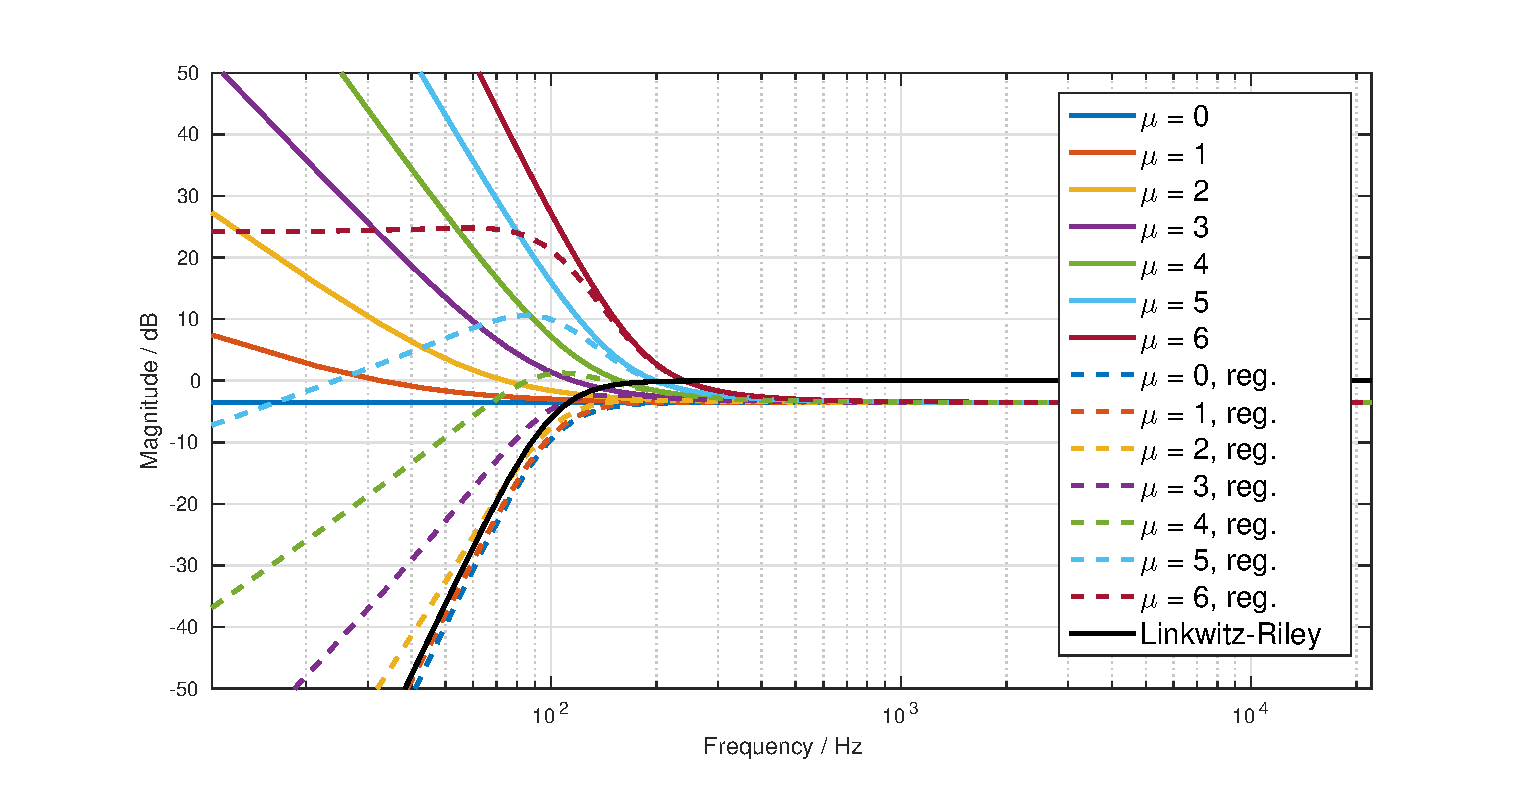
\includegraphics{fig}}%
    \gplfronttext
  \end{picture}%
\endgroup
